%!TEX program = xelatex
%!BIB program = bibtex

\documentclass[en,black,10pt,normal]{elegantnote}
\usepackage{float}
\usepackage{hyperref}

\newcommand{\upcite}[1]{\textsuperscript{\textsuperscript{\cite{#1}}}}

\title{Practical 3 Analyses of Sequence Characteristics}
\author{WenYuan Jiang\\ID: 1951510}
\institute{School of Life Science, Tongji University}
%\version{1.00}
\date{April 2, 2021}

\begin{document}

\maketitle

\section{What kind of results are analyzed by GENSCAN, ProtScale, TMpred and ProtParam respectively?}
\subsection{GENSCAN}
\texttt{GENESCAN} uses a general probabilistic model of the gene structure of human genomic sequences which incorporates descriptions of the basic transcriptional, 
translational and splicing signals, 
as well as length distributions and compositional features of exons, 
introns and intergenic regions.\upcite{burge1997prediction}

The input of \texttt{GENESCAN} is a DNA sequence (ASCII string, not a FASTA file) with a given threshold.
The output of \texttt{GENESCAN} is an ASCII text file that describes the possible introns and exons along with the possibilities (P).
The P value respresents how reliable a prediction is, and if $P>0.99$, the result is more likely to be true in real organisms.

\subsection{ProtScale}
\texttt{ProtScale} allows you to compute and represent the profile produced by any amino acid scale on a selected protein.

An amino acid scale is defined by a numerical value assigned to each type of amino acid. 
The most frequently used scales are the hydrophobicity or hydrophilicity scales and the secondary structure conformational parameters scales, 
but many other scales exist which are based on different chemical and physical properties of the amino acids. 
This program provides 57 predefined scales entered from the literature. \upcite{gasteiger2005protein}

The input of \texttt{ProtScale} is an amino acid sequence of a peptide, and it produces an ASCII text file that describes
the hydrophobicity or hydrophilicity scales of different regions of the peptide.

\subsection{TMpred}
The \texttt{TMpred} program makes a prediction of membrane-spanning regions and their orientation.\upcite{hofmann1993tmbase}

The input can be a sequence with no header information, or some id in the supported databases (see \url{https://embnet.vital-it.ch/software/format_help.html}).
The server then produces a html or ASCII file describing predictions of membrane-spanning regions and their orientation of the given sequence.


\subsection{ProtParam}
\texttt{ProtParam} is a tool which allows the computation of various physical and chemical parameters 
for a given protein stored in Swiss-Prot or TrEMBL or for a user entered protein sequence. 
The computed parameters include the molecular weight, theoretical pI, 
amino acid composition, atomic composition, extinction coefficient, estimated half-life, 
instability index, aliphatic index and grand average of hydropathicity (GRAVY).\upcite{gasteiger2005protein}

The input is a Swiss-Prot/TrEMBL accession number or an amino acid sequence (in one-letter code),
and the results will be in the form of ASCII file and a CSV file, with summarized physical and chemical parameters.

\section{Get SARS-cov-2 and ACE2 or your interested sequences from database.}
\subsection{SARS-cov-2 sequence}
The sequence is \texttt{NCBI Reference Sequence: NC\_045512.2}, fetched from \url{https://www.ncbi.nlm.nih.gov/nuccore/1798174254} on Apr 2, 2021.
The original sequence is published on \textit{Nature} by Wu et al.\upcite{wu2020new}
\subsection{ACE2 sequence}
The nucleotide sequence is fetched from \url{https://www.ncbi.nlm.nih.gov/nuccore/NG_012575.2} on Apr 2, 2021.
The protein sequence is \texttt{Angiotensin-converting enzyme 2}, fetched from \url{https://www.uniprot.org/uniprot/Q9BYF1} on Apr 2, 2021.

\subsection{Please predict the detail information of each sequence such as region of exons, promoter region, polyA region etc by tools. Compare the results with sequence information in Nucleotide.}

\subsubsection{Prediction of SARS-cov-2}
We will take CDS region as an example for the \textit{in silico} analysis of the sequence.
For more detailed results (like the polyA region etc), see the \texttt{Supplementary materials} section.

First we tried the \texttt{ORF finder}, but the results are not reasonable since there are 159 predicted ORFs.

The folllowing figure shows the prediction of exons of the SARS-cov-2 genome fetched from NCBI, 
along with Experimental data as the real situation. 

\begin{figure}[H]
    \centering
    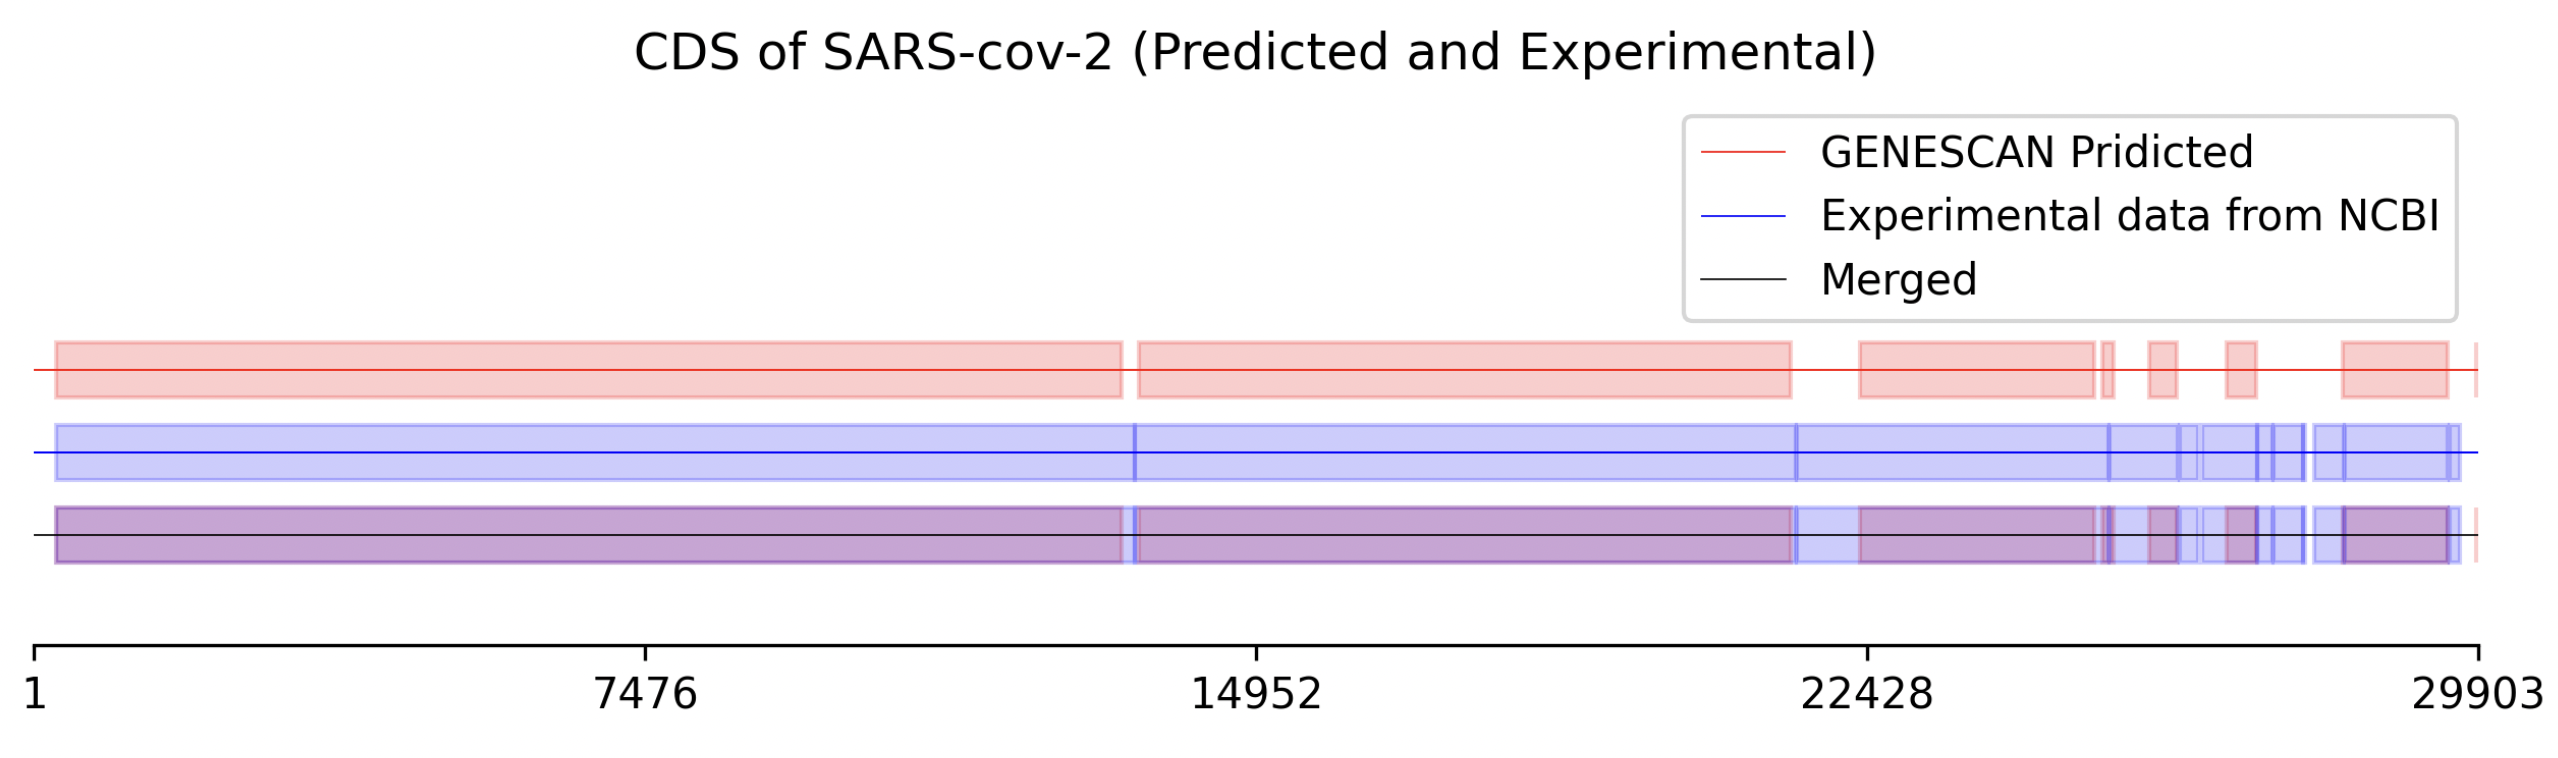
\includegraphics[width=1\textwidth]{Fig02}
    \caption{Exon Prediction of SARS-cov-2 using \texttt{GENSCAN}}
    \label{SARS}
\end{figure}

The tool used for prediction is \texttt{GENSCAN}, and parameters is on the table below.

\begin{table}[H]
    \caption{Parameters of GENSCAN}
    \centering
    \begin{tabular}{cc}
        \toprule
        Key&Value\\
        \midrule
        Organism&Vertebrate\\
        Suboptimal exon cutoff (optional)&0.10\\
        Print options&Predicted peptides only\\
        \bottomrule
    \end{tabular}
\end{table}

As can be seen on the figure above, \texttt{GENSCAN} is approximately correct in
predicting the CDS region of a sequence, and it skipped some of the CDS regions.

One reason for the error could be that the SARS-cov-2 is a virus while \texttt{GENSCAN}
dose not provide a parameter named virus in its Organism options. 
It is reasonable that virus have different patterns to organize their genome.



\subsubsection{Prediction of ACE2}
We will take exons as an example for the \textit{in silico} analysis of a sequence.
For more detailed results (like the polyA region etc), see the \texttt{Supplementary materials} section.

The folllowing figure shows the prediction of exons of the ACE2 gene fetched from NCBI, 
along with Experimental data as the real situation. 

\begin{figure}[H]
    \centering
    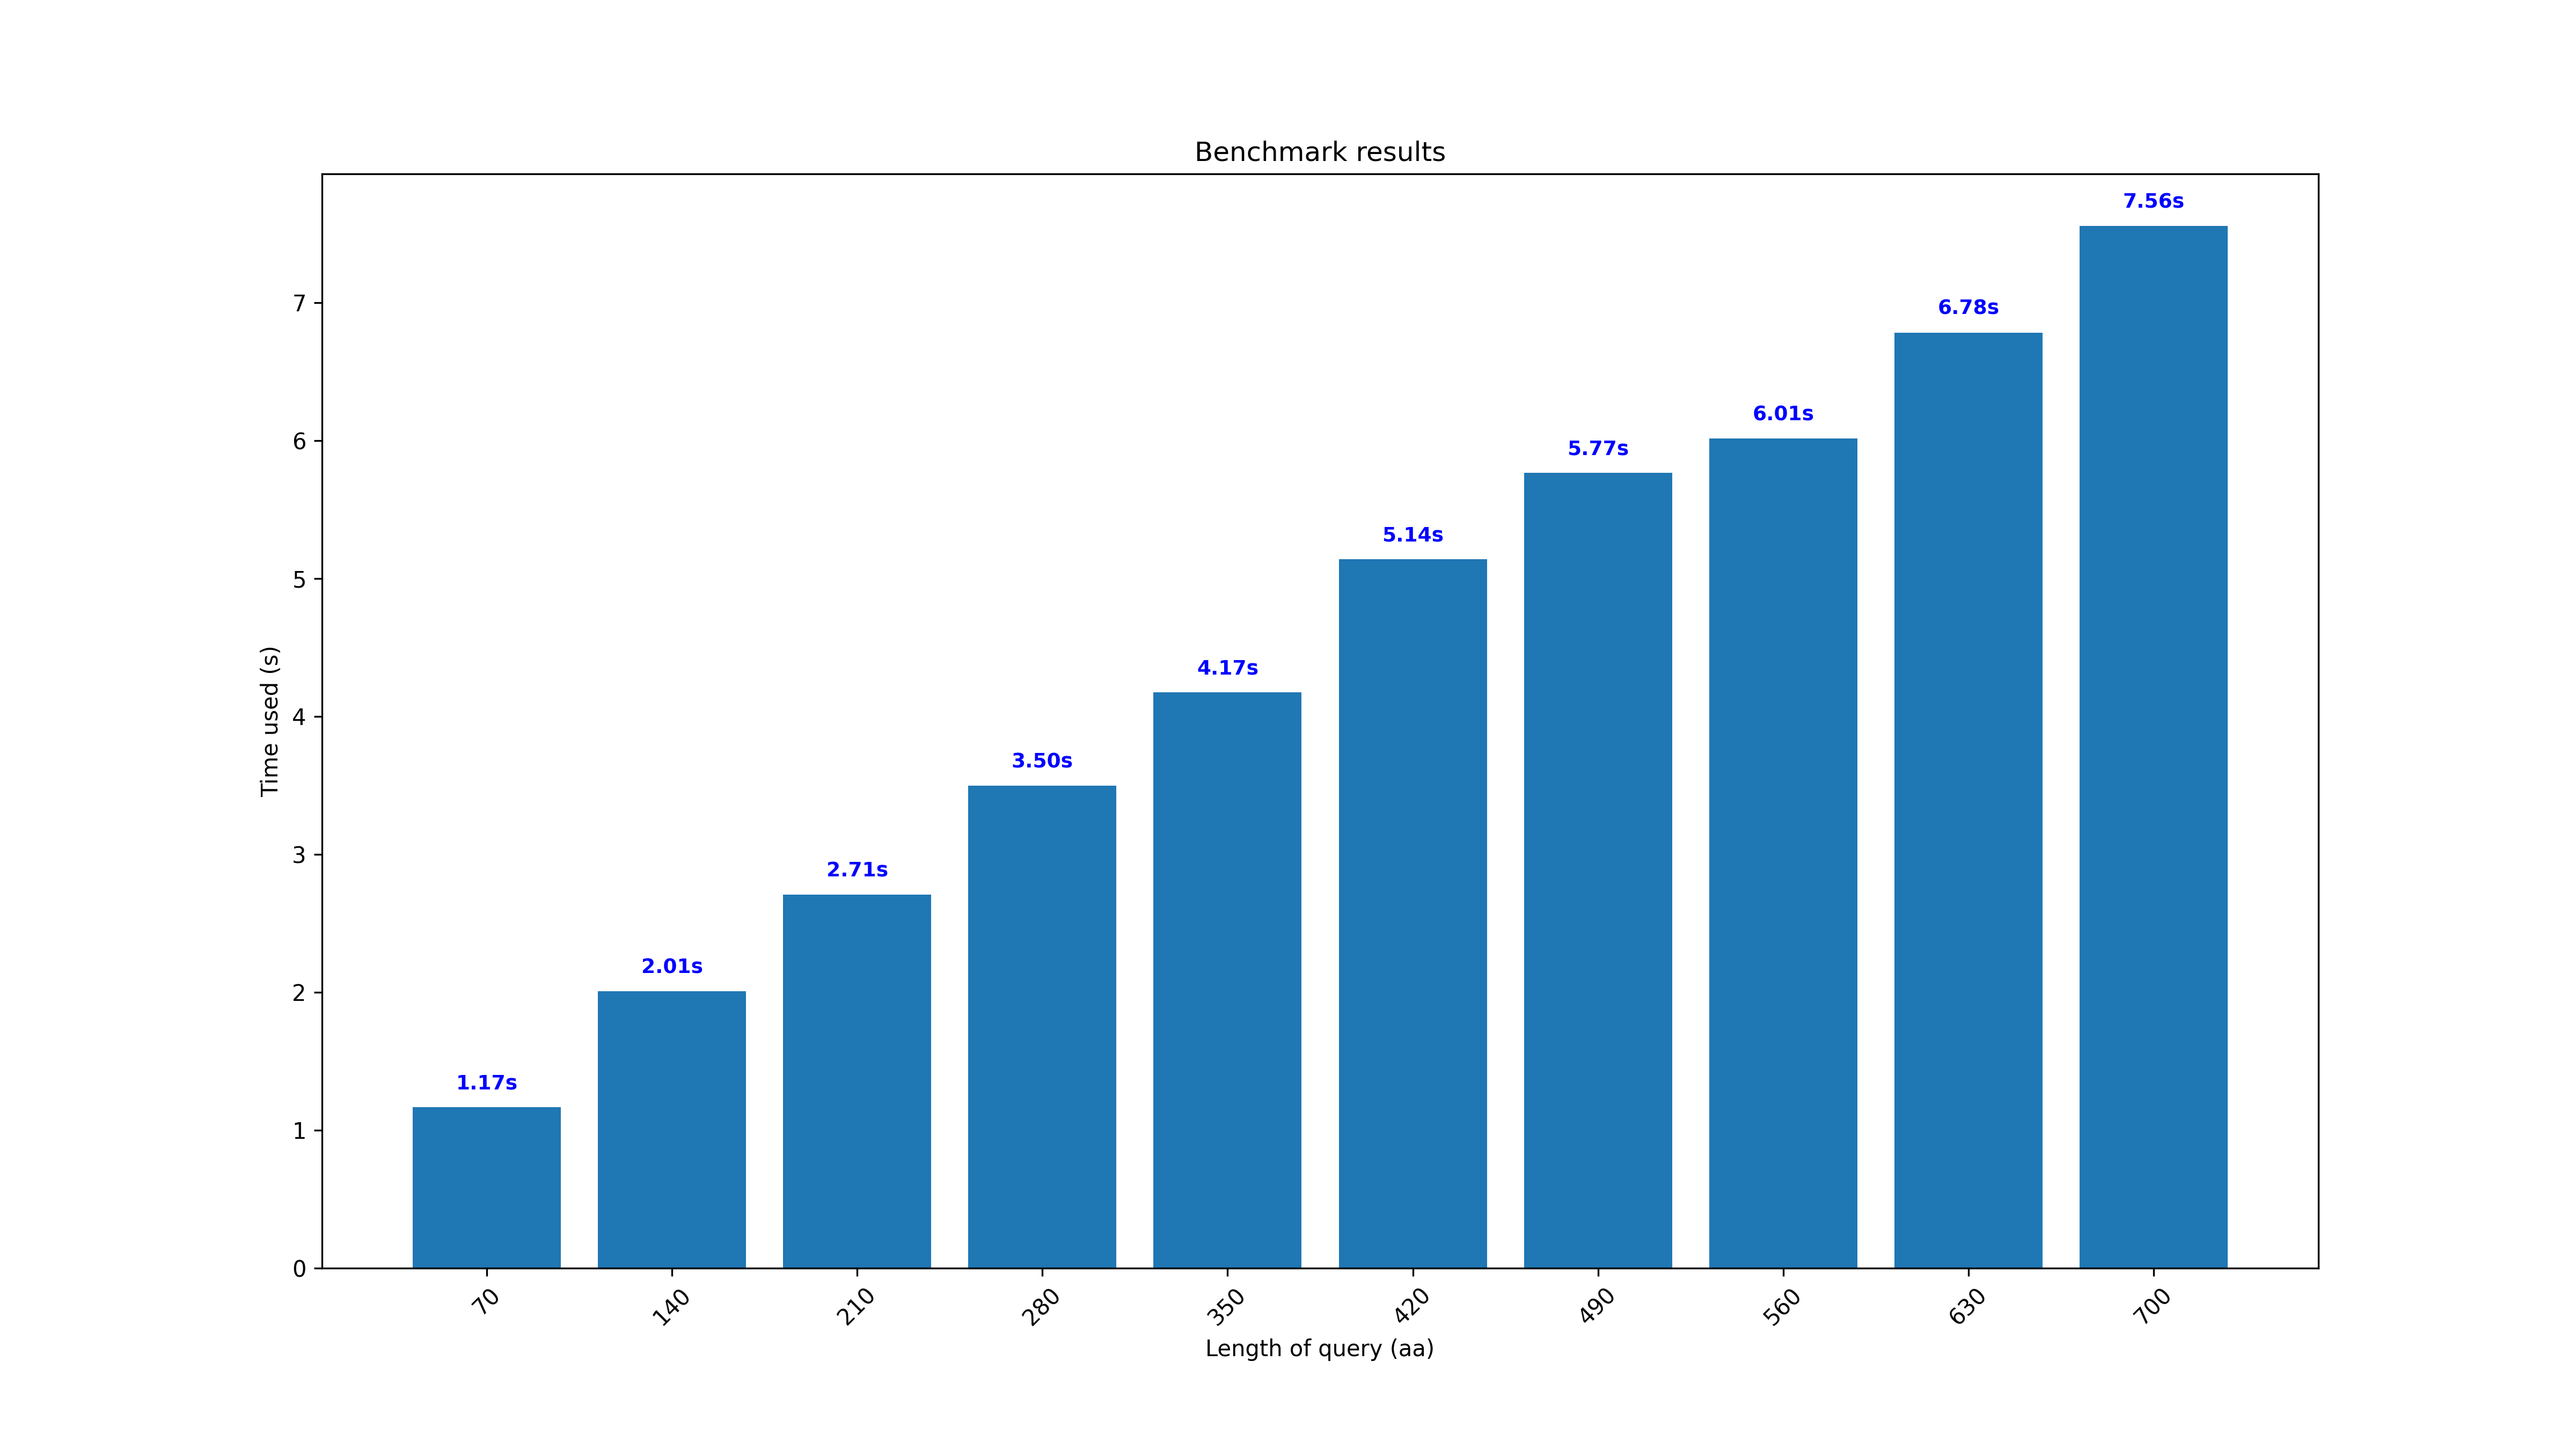
\includegraphics[width=1\textwidth]{Fig01}
    \caption{Exon Prediction of ACE2 using \texttt{GENSCAN}}
    \label{ACE2}
\end{figure}

The tool used for prediction is \texttt{GENSCAN}, and parameters is on the table below.

\begin{table}[H]
    \caption{Parameters of GENSCAN}
    \centering
    \begin{tabular}{cc}
        \toprule
        Key&Value\\
        \midrule
        Organism&Vertebrate\\
        Suboptimal exon cutoff (optional)&0.10\\
        Print options&Predicted peptides only\\
        \bottomrule
    \end{tabular}
\end{table}

As can be seen on the figure above, \texttt{GENSCAN} successfully predicted 14 of the 18 exons,
with high accuracy. The exons that \texttt{GENSCAN} failed to predict tend to be shorter, 
and with less significant features.

Using \texttt{ORF finder} gives out more than 300 ORFs, which is not desirable.

\subsection{Summarize the pros and cons of tools you used.}
\subsubsection{Advantage of ORF finder}
\texttt{ORF finder} is easy to implement and is fast enough to run on a long sequence.
Additionally, \texttt{ORF finder} has a simple mechanism, which is easy to understand.

\texttt{ORF finder} is also easy to use, and it provides a graphic view of the sequence.
\subsubsection{Limitation of ORF finder}
On most cases, \texttt{ORF finder} gives out numbers of uesless results.

\subsubsection{Advantages of GENSCAN}
This tool provides a relatively accurate prediction on an unknown sequence,
and the mathematics (probabilistic model) behind the tool is soild, unlike tools that 
uses deep learning.

\subsubsection{Limitations of GENSCAN}
The folllowing contents are collected from \url{http://hollywood.mit.edu/Limitations.html}
\paragraph{GENE NUMBER.} The number of genes predicted in a sequence is usually approximately correct but it may also happen that, for instance, a predicted gene splices together exons from two real genes, or vice versa.

\paragraph{ORGANISM.} The program was designed primarily to predict genes in human/vertebrate genomic sequences: accuracy may be lower for non-vertebrates. In particular, the vertebrate version of the program performs fairly well on Drosophila sequences and the maize and Arabidopsis versions perform fairly well on their respective organisms, but the program version for C. elegans sequences is still in the experimental stages. Other organisms have not been systematically tested. For prokaryotic or yeast sequences, the programs Glimmer, developed by Salzberg and colleagues, and/or GeneMark, developed by Borodovsky and McIninch, are recommended.

\paragraph{BIASES IN TEST SET.} The Burset/Guigó test set is undoubtedly biased toward short genes with relatively simple exon/intron structure: as a consequence, the statistics given in the tables on the accuracy page may not be completely representative of the performance of the programs on typical genomic DNA sequences.

\paragraph{EXON/FEATURE TYPE.} As a rule, internal exons are predicted more accurately than initial or terminal exons, and exons are predicted more accurately than polyadenylation or promoter signals. Predicted promoters, in particular, are not reliable. If promoters are of primary interest, you may wish to try Martin Reese's NNPP program.

\paragraph{PLANT SPLICE SIGNALS.} If identification of splice sites in plant pre-mRNAs is of primary interest, the SplicePredictor program developed by Brendel and colleagues is recommended.

\section{About ACE2\_human or your interested protein, Analyze the protein.}

Using \texttt{ProtParam}\upcite{gasteiger2005protein} to analyze the ACE2\_human protein (UniProtKB - Q9BYF1),
we get the folllowing result.

\subsection{Is this protein stable?}

\begin{lstlisting}[frame=single]
[OUTPUT]
...
    Instability index:

    The instability index (II) is computed to be 40.09
    This classifies the protein as unstable.
...
\end{lstlisting}

The prediction indicates that ACE2\_human protein is unstable under normal circumstances.
\subsection{PI}
Result given by \texttt{ProtParam}\upcite{gasteiger2005protein} of ACE2\_human protein (UniProtKB - Q9BYF1):

\begin{lstlisting}[frame=single]
[OUTPUT]
...
    Theoretical pI: 5.36
...
\end{lstlisting}
\subsection{Total number of negatively charged residues (Asp + Glu)}
Result given by \texttt{ProtParam}\upcite{gasteiger2005protein} of ACE2\_human protein (UniProtKB - Q9BYF1):

\begin{lstlisting}[frame=single]
[OUTPUT]
...
    Total number of negatively charged residues (Asp + Glu): 99
...
\end{lstlisting}

\subsection{Total number of positively charged residues (Arg + Lys)}
Result given by \texttt{ProtParam}\upcite{gasteiger2005protein} of ACE2\_human protein (UniProtKB - Q9BYF1):

\begin{lstlisting}[frame=single]
[OUTPUT]
...
    Total number of positively charged residues (Arg + Lys): 78
...
\end{lstlisting}

\subsection{Aliphatic index}
Result given by \texttt{ProtParam}\upcite{gasteiger2005protein} of ACE2\_human protein (UniProtKB - Q9BYF1):

\begin{lstlisting}[frame=single]
[OUTPUT]
...
    Aliphatic index: 80.55
...
\end{lstlisting}


\subsection{Grand average of hydropathicity (GRAVY)}
Result given by \texttt{ProtParam}\upcite{gasteiger2005protein} of ACE2\_human protein (UniProtKB - Q9BYF1):

\begin{lstlisting}[frame=single]
[OUTPUT]
...
    Grand average of hydropathicity (GRAVY): -0.375
...
\end{lstlisting}


\section{Predict hydrophobic regions and possible transmembrane regions of the protein. Compare and summarize the results.}
\subsection{Hydrophobic region prediction}

The tool used in hydrophobic region prediction is \texttt{ProtScale}\upcite{gasteiger2005protein}, 
and parameters are shown in the table below.

\begin{table}[H]
    \caption{Parameters of ProtScale}
    \centering
    \begin{tabular}{cc}
        \toprule
        Key&Value\\
        \midrule
        Amino acid scale&Hphob. / Kyte \& Doolittle\upcite{kyte1982simple} \\
        Window size&13\\
        Relative weight of the window edges compared to the window center (in \%)&20\\
        Weight variation model (if the relative weight at the edges is < 100\%)&linear\\
        Normalize the scale&No\\
        Query sequence:&Q9BYF1\\
        \bottomrule
    \end{tabular}
\end{table}
The result is shown in the figure below.
\begin{figure}[H]
    \centering
    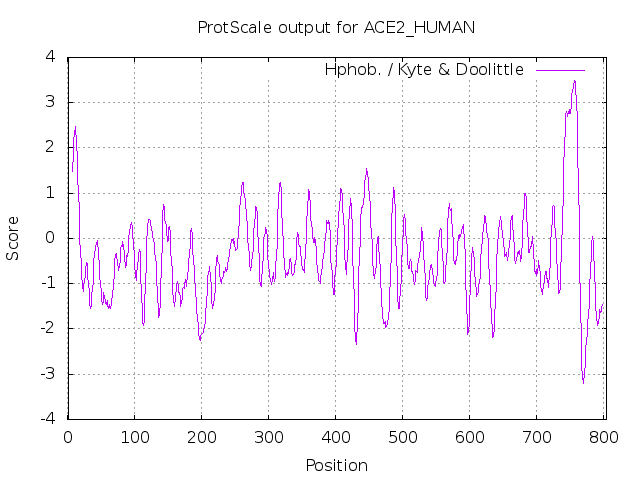
\includegraphics[width=1\textwidth]{pscale6481}
    \caption{Angiotensin-converting enzyme 2 precursor (EC 3.4.17.23). The computation has been carried out on the complete sequence (805 amino acids).Using the scale Hphob. / Kyte \& Doolittle\upcite{kyte1982simple}. Weights for window positions 1,..,13, using linear weight variation model.}
    \label{F-01}
\end{figure}

\subsection{Transmembrane region prediction}

The tool used in transmembrane region prediction is \texttt{TMpred}\upcite{hofmann1993tmbase}, 
and parameters are shown in the table below.

\begin{table}[H]
    \caption{Parameters of TMpred}
    \centering
    \begin{tabular}{cc}
        \toprule
        Key&Value\\
        \midrule
        Output format&ascii\\
        minimum&17\\
        maximum&33\\
        Input sequence format&SwissProt\_ID or AC\\
        Query sequence:&ACE2\_HUMAN\\
        \bottomrule
    \end{tabular}
\end{table}
The result is shown in the figure below.
\begin{figure}[H]
    \centering
    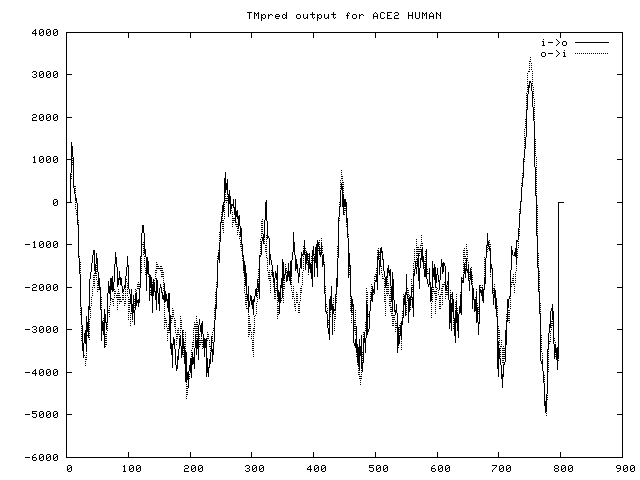
\includegraphics[width=1\textwidth]{TMPRED.5578.7790}
    \caption{TMpred output for ACE2\_HUMAN}
    \label{F-02}
\end{figure}

More detailed information of the prediction is listed in the \texttt{Supplementary materials} section.


\subsection{Comparison and summary}

According to the experiments done by Kowalczuk et al (2008), the human ACE2 protein is a 
\textbf{Single-pass type I membrane protein}, with its 
transmembrane helix on the 741 to 761 residues,\upcite{kowalczuk2008protein} which,
is close to one of the predictions given by \texttt{TMpred} (744 to 761).

This result is consistent with the predictions given by \texttt{ProtScale}, 
which indicates that the 740 to 770 of the sequence has a high hydrophobic score.

While other predictions given by \texttt{TMpred} is not correct, 
they are still consistent with the hydrophobic index. 
The real situation turns out that other hydrophobic regions belongs to a large extracellular domain,
which has more complicated functions.


\section{Discussions}

Since the 1980s when computers were first used in the field of life science,
many tools have been developed and published to help us
interprete and analyze sequences. Till today, most tools, even those 
in widespread use, can not give out ideal prediction, or meet the SOTA (State Of The Art) standard.
The tools used in this homework are the same.

The tools used to analyze sequence (nucleotide and protein) has different alogrithms behind them,
most of which uses classical statistical and probabilistic models. With more data feeded to
these alogrithms, these models are gaining much accuracy.

However, it is unlikely that a tool or an alogrithm can predict the properties of 
a sequence \textit{de novo}, that is, without extra information. Tools with high 
accuracy nowadays are mostly data-driven.

Even when we get a model that can predict the functions and properties of a sequence,
wet lab still matters for the validation of such tools, since life science 
is based on experiments rather than deduction.


\section{Supplementary materials}
\subsection{\texttt{GENSCAN} results of SARS-cov-2}
\begin{lstlisting}[frame=single]
[OUTPUT]
GENSCAN 1.0	Date run:  3-Apr-121	Time: 01:37:07



Sequence /tmp/04_03_21-01:37:05.fasta : 29903 bp : 37.97% C+G : Isochore 1 ( 0 - 43 C+G%)



Parameter matrix: HumanIso.smat



Predicted genes/exons:



Gn.Ex Type S .Begin ...End .Len Fr Ph I/Ac Do/T CodRg P.... Tscr..

----- ---- - ------ ------ ---- -- -- ---- ---- ----- ----- ------



 1.01 Init +    266  13304 13039  1  1   83  115  6398 0.263 629.73

 1.02 Intr +  13514  21490 7977  0  0   24   69  3498 0.375 327.97

 1.03 Intr +  22332  25203 2872  1  1   87   43  1545 0.754 136.29

 1.04 Intr +  25298  25444  147  2  0   45   62   108 0.828   2.33

 1.05 Intr +  25878  26216  339  0  0   41   52   320 0.973  17.36

 1.06 Intr +  26825  27187  363  2  0   94   98   384 0.942  33.37

 1.07 Term +  28249  29533 1285  1  1   45   37  1343 0.991 114.96

 1.08 PlyA +  29871  29876    6                              -0.45





Suboptimal exons with probability > 0.010



Exnum Type S .Begin ...End .Len Fr Ph B/Ac Do/T CodRg P.... Tscr..

----- ---- - ------ ------ ---- -- -- ---- ---- ----- ----- ------



S.001 Init +    266   6617 6352  1  1   83    8  4732 0.032 452.31

S.002 Init +    266   6641 6376  1  1   83  -26  4758 0.018 451.51

S.003 Init +    266   6716 6451  1  1   83  -46  4770 0.011 450.72

S.004 Init +    266   6741 6476  1  2   83  -11  4771 0.282 454.32

S.005 Init +    266   6884 6619  1  1   83   24  4738 0.147 454.52

S.006 Init +    266  10958 10693  1  1   83   36  5573 0.040 539.29

S.007 Init +    266  10997 10732  1  1   83   48  5559 0.035 539.09

S.008 Init +    266  13385 13120  1  1   83   80  6388 0.011 625.23

S.009 Init +    266  13479 13214  1  2   83   78  6438 0.124 630.03

S.010 Intr +   7321  13304 5984  1  2   54  115  1854 0.014 171.14

S.011 Intr +   7401  10958 3558  1  0   45   36  1058 0.014  82.70

S.012 Intr +   7401  10997 3597  1  0   45   48  1044 0.013  82.50

S.013 Intr +   7401  13304 5904  1  0   45  115  1883 0.094 173.14

S.014 Intr +   7401  13479 6079  1  1   45   78  1923 0.045 173.44

S.015 Intr +   7411  13304 5894  1  2  -11  115  1923 0.018 171.54

S.016 Intr +   7470  13304 5835  1  0   -2  115  1904 0.016 170.54

S.017 Intr +   7516  13304 5789  1  2   10  115  1916 0.048 172.94

S.018 Intr +   7516  13479 5964  1  0   10   78  1956 0.023 173.24

S.019 Intr +   7651  13304 5654  1  2   29  115  1900 0.059 173.23

S.020 Intr +   7651  13479 5829  1  0   29   78  1940 0.028 173.54

S.021 Intr +  11208  11534  327  1  0   80   57    89 0.022  -0.25

S.022 Intr +  11208  13304 2097  1  0   80  115   978 0.052  86.07

S.023 Intr +  11208  13479 2272  1  1   80   78  1018 0.025  86.38

S.024 Intr +  11355  11534  180  1  0   22   57    97 0.013  -1.08

S.025 Intr +  11625  13304 1680  1  0   69  115   969 0.039  84.07

S.026 Intr +  11625  13479 1855  1  1   69   78  1009 0.019  84.37

S.027 Intr +  11709  13304 1596  1  0   33  115   974 0.011  82.25

S.028 Intr +  13371  13479  109  1  1   17   78    70 0.040  -2.68

S.029 Intr +  13514  21424 7911  0  0   24   36  3505 0.062 325.37

S.030 Intr +  13514  21451 7938  0  0   24   43  3515 0.201 327.07

S.031 Intr +  13539  21424 7886  0  2   49   36  3467 0.033 324.07

S.032 Intr +  13539  21451 7913  0  2   49   43  3477 0.108 325.77

S.033 Intr +  13539  21490 7952  0  2   49   69  3460 0.201 326.67

S.034 Intr +  21894  22025  132  1  0   30   87    11 0.027  -5.10

S.035 Intr +  21894  25203 3310  1  1   30   43  1543 0.012 130.39

S.036 Intr +  22233  25203 2971  1  1   52   43  1520 0.012 130.29

S.037 Intr +  22332  25176 2845  1  1   87   16  1551 0.176 134.19

S.038 Intr +  25727  25752   26  2  2   74   41    22 0.018  -7.15

S.039 Intr +  25907  26216  310  0  1   80   52   287 0.021  18.75

S.040 Intr +  26738  27187  450  2  0   84   98   370 0.048  29.09





Predicted peptide sequence(s):





>/tmp/04_03_21-01:37:05.fasta|GENSCAN_predicted_peptide_1|8673_aa

MESLVPGFNEKTHVQLSLPVLQVRDVLVRGFGDSVEEVLSEARQHLKDGTCGLVEVEKGV

LPQLEQPYVFIKRSDARTAPHGHVMVELVAELEGIQYGRSGETLGVLVPHVGEIPVAYRK

VLLRKNGNKGAGGHSYGADLKSFDLGDELGTDPYEDFQENWNTKHSSGVTRELMRELNGG

AYTRYVDNNFCGPDGYPLECIKDLLARAGKASCTLSEQLDFIDTKRGVYCCREHEHEIAW

YTERSEKSYELQTPFEIKLAKKFDTFNGECPNFVFPLNSIIKTIQPRVEKKKLDGFMGRI

RSVYPVASPNECNQMCLSTLMKCDHCGETSWQTGDFVKATCEFCGTENLTKEGATTCGYL

PQNAVVKIYCPACHNSEVGPEHSLAEYHNESGLKTILRKGGRTIAFGGCVFSYVGCHNKC

AYWVPRASANIGCNHTGVVGEGSEGLNDNLLEILQKEKVNINIVGDFKLNEEIAIILASF

SASTSAFVETVKGLDYKAFKQIVESCGNFKVTKGKAKKGAWNIGEQKSILSPLYAFASEA

ARVVRSIFSRTLETAQNSVRVLQKAAITILDGISQYSLRLIDAMMFTSDLATNNLVVMAY

ITGGVVQLTSQWLTNIFGTVYEKLKPVLDWLEEKFKEGVEFLRDGWEIVKFISTCACEIV

GGQIVTCAKEIKESVQTFFKLVNKFLALCADSIIIGGAKLKALNLGETFVTHSKGLYRKC

VKSREETGLLMPLKAPKEIIFLEGETLPTEVLTEEVVLKTGDLQPLEQPTSEAVEAPLVG

TPVCINGLMLLEIKDTEKYCALAPNMMVTNNTFTLKGGAPTKVTFGDDTVIEVQGYKSVN

ITFELDERIDKVLNEKCSAYTVELGTEVNEFACVVADAVIKTLQPVSELLTPLGIDLDEW

SMATYYLFDESGEFKLASHMYCSFYPPDEDEEEGDCEEEEFEPSTQYEYGTEDDYQGKPL

EFGATSAALQPEEEQEEDWLDDDSQQTVGQQDGSEDNQTTTIQTIVEVQPQLEMELTPVV

QTIEVNSFSGYLKLTDNVYIKNADIVEEAKKVKPTVVVNAANVYLKHGGGVAGALNKATN

NAMQVESDDYIATNGPLKVGGSCVLSGHNLAKHCLHVVGPNVNKGEDIQLLKSAYENFNQ

HEVLLAPLLSAGIFGADPIHSLRVCVDTVRTNVYLAVFDKNLYDKLVSSFLEMKSEKQVE

QKIAEIPKEEVKPFITESKPSVEQRKQDDKKIKACVEEVTTTLEETKFLTENLLLYIDIN

GNLHPDSATLVSDIDITFLKKDAPYIVGDVVQEGVLTAVVIPTKKAGGTTEMLAKALRKV

PTDNYITTYPGQGLNGYTVEEAKTVLKKCKSAFYILPSIISNEKQEILGTVSWNLREMLA

HAEETRKLMPVCVETKAIVSTIQRKYKGIKIQEGVVDYGARFYFYTSKTTVASLINTLND

LNETLVTMPLGYVTHGLNLEEAARYMRSLKVPATVSVSSPDAVTAYNGYLTSSSKTPEEH

FIETISLAGSYKDWSYSGQSTQLGIEFLKRGDKSVYYTSNPTTFHLDGEVITFDNLKTLL

SLREVRTIKVFTTVDNINLHTQVVDMSMTYGQQFGPTYLDGADVTKIKPHNSHEGKTFYV

LPNDDTLRVEAFEYYHTTDPSFLGRYMSALNHTKKWKYPQVNGLTSIKWADNNCYLATAL

LTLQQIELKFNPPALQDAYYRARAGEAANFCALILAYCNKTVGELGDVRETMSYLFQHAN

LDSCKRVLNVVCKTCGQQQTTLKGVEAVMYMGTLSYEQFKKGVQIPCTCGKQATKYLVQQ

ESPFVMMSAPPAQYELKHGTFTCASEYTGNYQCGHYKHITSKETLYCIDGALLTKSSEYK

GPITDVFYKENSYTTTIKPVTYKLDGVVCTEIDPKLDNYYKKDNSYFTEQPIDLVPNQPY

PNASFDNFKFVCDNIKFADDLNQLTGYKKPASRELKVTFFPDLNGDVVAIDYKHYTPSFK

KGAKLLHKPIVWHVNNATNKATYKPNTWCIRCLWSTKPVETSNSFDVLKSEDAQGMDNLA

CEDLKPVSEEVVENPTIQKDVLECNVKTTEVVGDIILKPANNSLKITEEVGHTDLMAAYV

DNSSLTIKKPNELSRVLGLKTLATHGLAAVNSVPWDTIANYAKPFLNKVVSTTTNIVTRC

LNRVCTNYMPYFFTLLLQLCTFTRSTNSRIKASMPTTIAKNTVKSVGKFCLEASFNYLKS

PNFSKLINIIIWFLLLSVCLGSLIYSTAALGVLMSNLGMPSYCTGYREGYLNSTNVTIAT

YCTGSIPCSVCLSGLDSLDTYPSLETIQITISSFKWDLTAFGLVAEWFLAYILFTRFFYV

LGLAAIMQLFFSYFAVHFISNSWLMWLIINLVQMAPISAMVRMYIFFASFYYVWKSYVHV

VDGCNSSTCMMCYKRNRATRVECTTIVNGVRRSFYVYANGGKGFCKLHNWNCVNCDTFCA

GSTFISDEVARDLSLQFKRPINPTDQSSYIVDSVTVKNGSIHLYFDKAGQKTYERHSLSH

FVNLDNLRANNTKGSLPINVIVFDGKSKCEESSAKSASVYYSQLMCQPILLLDQALVSDV

GDSAEVAVKMFDAYVNTFSSTFNVPMEKLKTLVATAEAELAKNVSLDNVLSTFISAARQG

FVDSDVETKDVVECLKLSHQSDIEVTGDSCNNYMLTYNKVENMTPRDLGACIDCSARHIN

AQVAKSHNIALIWNVKDFMSLSEQLRKQIRSAAKKNNLPFKLTCATTRQVVNVVTTKIAL

KGGKIVNNWLKQLIKVTLVFLFVAAIFYLITPVHVMSKHTDFSSEIIGYKAIDGGVTRDI

ASTDTCFANKHADFDTWFSQRGGSYTNDKACPLIAAVITREVGFVVPGLPGTILRTTNGD

FLHFLPRVFSAVGNICYTPSKLIEYTDFATSACVLAAECTIFKDASGKPVPYCYDTNVLE

GSVAYESLRPDTRYVLMDGSIIQFPNTYLEGSVRVVTTFDSEYCRHGTCERSEAGVCVST

SGRWVLNNDYYRSLPGVFCGVDAVNLLTNMFTPLIQPIGALDISASIVAGGIVAIVVTCL

AYYFMRFRRAFGEYSHVVAFNTLLFLMSFTVLCLTPVYSFLPGVYSVIYLYLTFYLTNDV

SFLAHIQWMVMFTPLVPFWITIAYIICISTKHFYWFFSNYLKRRVVFNGVSFSTFEEAAL

CTFLLNKEMYLKLRSDVLLPLTQYNRYLALYNKYKYFSGAMDTTSYREAACCHLAKALND

FSNSGSDVLYQPPQTSITSAVLQSGFRKMAFPSGKVEGCMVQVTCGTTTLNGLWLDDVVY

CPRHVICTSEDMLNPNYEDLLIRKSNHNFLVQAGNVQLRVIGHSMQNCVLKLKVDTANPK

TPKYKFVRIQPGQTFSVLACYNGSPSGVYQCAMRPNFTIKGSFLNGSCGSVGFNIDYDCV

SFCYMHHMELPTGVHAGTDLEGNFYGPFVDRQTAQAAGTDTTITVNVLAWLYAAVINGDR

WFLNRFTTTLNDFNLVAMKYNYEPLTQDHVDILGPLSAQTGIAVLDMCASLKELLQNGMN

GRTILGSALLEDEFTPFDVVRQCSGVTFQSAVKRTIKGTHHWLLLTILTSLLVLVQSTQW

SLFFFLYENAFLPFAMGIIAMSAFAMMFVKHKHAFLCLFLLPSLATVAYFNMVYMPASWV

MRIMTWLDMVDTSLSGFKLKDCVMYASAVVLLILMTARTVYDDGARRVWTLMNVLTLVYK

VYYGNALDQAISMWALIISVTSNYSGVVTTVMFLARGIVFMCVEYCPIFFITGNTLQCIM

LVYCFLGYFCTCYFGLFCLLNRYFRLTLGVYDYLVSTQEFRYMNSQGLLPPKNSIDAFKL

NIKLLGVGGKPCIKVATVQSKMSDVKCTSVVLLSVLQQLRVESSSKLWAQCVQLHNDILL

AKDTTEAFEKMVSLLSVLLSMQGAVDINKLCEEMLDNRATLQAIASEFSSLPSYAAFATA

QEAYEQAVANGDSEVVLKKLKKSLNVAKSEFDRDAAMQRKLEKMADQAMTQMYKQARSED

KRAKVTSAMQTMLFTMLRKLDNDALNNIINNARDGCVPLNIIPLTTAAKLMVVIPDYNTY

KNTCDGTTFTYASALWEIQQVVDADSKIVQLSEISMDNSPNLAWPLIVTALRANSAVKLQ

NNELSPVALRQMSCAAGTTQTACTDDNALAYYNTTKGGRFVLALLSDLQDLKWARFPKSD

GTGTIYTELEPPCRFVTDTPKGPKVKYLYFIKGLNNLNRGMVLGSLAATVRLQAGNATEV

PANSTVLSFCAFAVDAAKAYKDYLASGGQPITNCVKMLCTHTGTGQAITVTPEANMDQES

FGGASCCLYCRCHIDHPNPKGFCDLKGTSTDVVYRAFDIYNDKVAGFAKFLKTNCCRFQE

KDEDDNLIDSYFVVKRHTFSNYQHEETIYNLLKDCPAVAKHDFFKFRIDGDMVPHISRQR

LTKYTMADLVYALRHFDEGNCDTLKEILVTYNCCDDDYFNKKDWYDFVENPDILRVYANL

GERVRQALLKTVQFCDAMRNAGIVGVLTLDNQDLNGNWYDFGDFIQTTPGSGVPVVDSYY

SLLMPILTLTRALTAESHVDTDLTKPYIKWDLLKYDFTEERLKLFDRYFKYWDQTYHPNC

VNCLDDRCILHCANFNVLFSTVFPPTSFGPLVRKIFVDGVPFVVSTGYHFRELGVVHNQD

VNLHSSRLSFKELLVYAADPAMHAASGNLLLDKRTTCFSVAALTNNVAFQTVKPGNFNKD

FYDFAVSKGFFKEGSSVELKHFFFAQDGNAAISDYDYYRYNLPTMCDIRQLLFVVEVVDK

YFDCYDGGCINANQVIVNNLDKSAGFPFNKWGKARLYYDSMSYEDQDALFAYTKRNVIPT

ITQMNLKYAISAKNRARTVAGVSICSTMTNRQFHQKLLKSIAATRGATVVIGTSKFYGGW

HNMLKTVYSDVENPHLMGWDYPKCDRAMPNMLRIMASLVLARKHTTCCSLSHRFYRLANE

CAQVLSEMVMCGGSLYVKPGGTSSGDATTAYANSVFNICQAVTANVNALLSTDGNKIADK

YVRNLQHRLYECLYRNRDVDTDFVNEFYAYLRKHFSMMILSDDAVVCFNSTYASQGLVAS

IKNFKSVLYYQNNVFMSEAKCWTETDLTKGPHEFCSQHTMLVKQGDDYVYLPYPDPSRIL

GAGCFVDDIVKTDGTLMIERFVSLAIDAYPLTKHPNQEYADVFHLYLQYIRKLHDELTGH

MLDMYSVMLTNDNTSRYWEPEFYEAMYTPHTVLQAVGACVLCNSQTSLRCGACIRRPFLC

CKCCYDHVISTSHKLVLSVNPYVCNAPGCDVTDVTQLYLGGMSYYCKSHKPPISFPLCAN

GQVFGLYKNTCVGSDNVTDFNAIATCDWTNAGDYILANTCTERLKLFAAETLKATEETFK

LSYGIATVREVLSDRELHLSWEVGKPRPPLNRNYVFTGYRVTKNSKVQIGEYTFEKGDYG

DAVVYRGTTTYKLNVGDYFVLTSHTVMPLSAPTLVPQEHYVRITGLYPTLNISDEFSSNV

ANYQKVGMQKYSTLQGPPGTGKSHFAIGLALYYPSARIVYTACSHAAVDALCEKALKYLP

IDKCSRIIPARARVECFDKFKVNSTLEQYVFCTVNALPETTADIVVFDEISMATNYDLSV

VNARLRAKHYVYIGDPAQLPAPRTLLTKGTLEPEYFNSVCRLMKTIGPDMFLGTCRRCPA

EIVDTVSALVYDNKLKAHKDKSAQCFKMFYKGVITHDVSSAINRPQIGVVREFLTRNPAW

RKAVFISPYNSQNAVASKILGLPTQTVDSSQGSEYDYVIFTQTTETAHSCNVNRFNVAIT

RAKVGILCIMSDRDLYDKLQFTSLEIPRRNVATLQAENVTGLFKDCSKVITGLHPTQAPT

HLSVDTKFKTEGLCVDIPGIPKDMTYRRLISMMGFKMNYQVNGYPNMFITREEAIRHVRA

WIGFDVEGCHATREAVGTNLPLQLGFSTGVNLVAVPTGYVDTPNNTDFSRVSAKPPPGDQ

FKHLIPLMYKGLPWNVVRIKIVQMLSDTLKNLSDRVVFVLWAHGFELTSMKYFVKIGPER

TCCLCDRRATCFSTASDTYACWHHSIGFDYVYNPFMIDVQQWGFTGNLQSNHDLYCQVHG

NAHVASCDAIMTRCLAVHECFVKRVDWTIEYPIIGDELKINAACRKVQHMVVKAALLADK

FPVLHDIGNPKAIKCVPQADVEWKFYDAQPCSDKAYKIEELFYSYATHSDKFTDGVCLFW

NCNVDRYPANSIVCRFDTRVLSNLNLPGCDGGSLYVNKHAFHTPAFDKSAFVNLKQLPFF

YYSDSPCESHGKQVVSDIDYVPLKSATCITRCNLGGAVCRHHANEYRLYLDAYNMMISAG

FSLWVYKQFDTYNLWNTFTRLQSLENVAFNVVNKGHFDGQQGEVPVSIINNTVYTKVDGV

DVELFENKTTLPVNVAFELWAKRNIKPVPEVKILNNLGVDIAANTVIWDYKRDAPAHIST

IGVCSMTDIAKKPTETICAPLTVFFDGRVDGQVDLFRNARNGVLITEGSVKGLQPSVGPK

QASLNGVTLIGEAVKTQFNYYKKVDGVVQQLPETYFTQSRNLQEFKPRSQMEIDFLELAM

DEFIERYKLEGYAFEHIVYGDFSHSQLGGLHLLIGLAKRFKESPFELEDFIPMDSTVKNY

FITDAQTGSSKCVCSVIDLLLDDFVEIIKSQDLSVVSKVVKVTIDYTEISFMLWCKDGHV

ETFYPKLQSSQAWQPGVAMPNLYKMQRMLLEKCDLQNYGDSATLPKGIMMNVAKYTQLCQ

YLNTLTLAVPYNMRVIHFGAGSDKGVAPGTAVLRQWLPTGTLLVDSDLNDFVSDADSTLI

GDCATVHTANKWDLIISDMYDPKTKNVTKENDSKEGFFTYICGFIQQKLALGGSVAIKIT

EHSWNADLYKLMGHFAWWTAFVTNVNASSSEAFLIGCNYLGKPREQIDGYVMHANYIFWR

NTNPIQLSSYSLFDMSKFPLKLRGTAVMSLKEGQINDMILSLLSKGWTAGAAAYYVGYLQ

PRTFLLKYNENGTITDAVDCALDPLSETKCTLKSFTVEKGIYQTSNFRVQPTESIVRFPN

ITNLCPFGEVFNATRFASVYAWNRKRISNCVADYSVLYNSASFSTFKCYGVSPTKLNDLC

FTNVYADSFVIRGDEVRQIAPGQTGKIADYNYKLPDDFTGCVIAWNSNNLDSKVGGNYNY

LYRLFRKSNLKPFERDISTEIYQAGSTPCNGVEGFNCYFPLQSYGFQPTNGVGYQPYRVV

VLSFELLHAPATVCGPKKSTNLVKNKCVNFNFNGLTGTGVLTESNKKFLPFQQFGRDIAD

TTDAVRDPQTLEILDITPCSFGGVSVITPGTNTSNQVAVLYQDVNCTEVPVAIHADQLTP

TWRVYSTGSNVFQTRAGCLIGAEHVNNSYECDIPIGAGICASYQTQTNSPRRARSVASQS

IIAYTMSLGAENSVAYSNNSIAIPTNFTISVTTEILPVSMTKTSVDCTMYICGDSTECSN

LLLQYGSFCTQLNRALTGIAVEQDKNTQEVFAQVKQIYKTPPIKDFGGFNFSQILPDPSK

PSKRSFIEDLLFNKVTLADAGFIKQYGDCLGDIAARDLICAQKFNGLTVLPPLLTDEMIA

QYTSALLAGTITSGWTFGAGAALQIPFAMQMAYRFNGIGVTQNVLYENQKLIANQFNSAI

GKIQDSLSSTASALGKLQDVVNQNAQALNTLVKQLSSNFGAISSVLNDILSRLDKVEAEV

QIDRLITGRLQSLQTYVTQQLIRAAEIRASANLAATKMSECVLGQSKRVDFCGKGYHLMS

FPQSAPHGVVFLHVTYVPAQEKNFTTAPAICHDGKAHFPREGVFVSNGTHWFVTQRNFYE

PQIITTDNTFVSGNCDVVIGIVNNTVYDPLQPELDSFKEELDKYFKNHTSPDVDLGDISG

INASVVNIQKEIDRLNEVAKNLNESLIDLQELGKYEQYIKWPWAVVLVDPAANLMKTTLS

QCSKESNYITHKRTYGFVYENLHNWNCNFEASVTSSIVITSGDGTTSPISEHDYQIGGYT

EKWESGVKDCVVLHSYFTSDYYQLYSTQLSTDTGVEHVTFFIYNKIVDEPEEHVQIHTID

GSSGVVNPVMEPIYDEPTTTTSVPLLFARTRSMWSFNPETNILLNVPLHGTILTRPLLES

ELVIGAVILRGHLRIAGHHLGRCDIKDLPKEITVATSRTLSYYKLGASQRVAGDSGFAAY

SRYRIGNYKLNTDHSSSSDNIALLVQFHLNEQTKMSDNGPQNQRNAPRITFGGPSDSTGS

NQNGERSGARSKQRRPQGLPNNTASWFTALTQHGKEDLKFPRGQGVPINTNSSPDDQIGY

YRRATRRIRGGDGKMKDLSPRWYFYYLGTGPEAGLPYGANKDGIIWVATEGALNTPKDHI

GTRNPANNAAIVLQLPQGTTLPKGFYAEGSRGGSQASSRSSSRSRNSSRNSTPGSSRGTS

PARMAGNGGDAALALLLLDRLNQLESKMSGKGQQQQGQTVTKKSAAEASKKPRQKRTATK

AYNVTQAFGRRGPEQTQGNFGDQELIRQGTDYKHWPQIAQFAPSASAFFGMSRIGMEVTP

SGTWLTYTGAIKLDDKDPNFKDQVILLNKHIDAYKTFPPTEPKKDKKKKADETQALPQRQ

KKQQTVTLLPAADLDDFSKQLQQSMSSADSTQA
\end{lstlisting}


\subsection{\texttt{GENSCAN} results of ACE2}
\begin{lstlisting}[frame=single]
[OUTPUT]
GENSCAN 1.0	Date run:  3-Apr-121	Time: 01:10:13



Sequence /tmp/04_03_21-01:10:13.fasta : 39928 bp : 38.31% C+G : Isochore 1 ( 0 - 43 C+G%)



Parameter matrix: HumanIso.smat



Predicted genes/exons:



Gn.Ex Type S .Begin ...End .Len Fr Ph I/Ac Do/T CodRg P.... Tscr..

----- ---- - ------ ------ ---- -- -- ---- ---- ----- ----- ------



 1.01 Intr +     79    235  157  1  1   67  101   181 0.682  16.39

 1.02 Intr +   5958   6116  159  2  0  104   87   181 0.935  18.86

 1.03 Intr +   8639   8732   94  1  1   80   96    45 0.929   3.12

 1.04 Intr +   9105   9248  144  1  0   23   97    68 0.567   0.53

 1.05 Intr +  11505  11617  113  1  2  -22   99   179 0.990   7.18

 1.06 Intr +  13103  13208  106  1  1   85   91    36 0.888   2.47

 1.07 Intr +  15389  15486   98  0  2   61   91    39 0.554   0.31

 1.08 Intr +  19571  19740  170  1  2   89   72   129 0.982   9.22

 1.09 Intr +  22646  22872  227  2  2   82   56   170 0.969   9.91

 1.10 Intr +  25151  25295  145  0  1   84  100    24 0.556   1.62

 1.11 Intr +  28638  28760  123  0  0   99   44   125 0.921   7.98

 1.12 Intr +  29165  29337  173  2  2   68   84    71 0.695   3.36

 1.13 Intr +  34522  34708  187  2  1   72   61    66 0.193   0.13

 1.14 Intr +  36743  36937  195  2  0   71  100   219 0.967  19.01

 1.15 Term +  38948  39056  109  2  1   73   43   118 0.949   2.80

 1.16 PlyA +  39905  39910    6                               1.05





Suboptimal exons with probability > 0.010



Exnum Type S .Begin ...End .Len Fr Ph B/Ac Do/T CodRg P.... Tscr..

----- ---- - ------ ------ ---- -- -- ---- ---- ----- ----- ------



S.001 Intr +     44    235  192  1  0   45  101   172 0.064  12.97

S.002 Init +     50    235  186  1  0   67  101   167 0.250  14.94

S.003 Intr +   5137   5166   30  0  0   80   75    -7 0.023  -5.39

S.004 Term +   5958   6128  171  2  0  104   47   221 0.059  16.44

S.005 Intr +   7264   7374  111  0  0  -69   91   116 0.050  -4.14

S.006 Init +   8660   8732   73  1  1   46   96    62 0.032   4.08

S.007 Init +   9119   9248  130  1  1   64   97    62 0.037   5.06

S.008 Intr +  13884  13927   44  1  2   60   24    66 0.011  -5.56

S.009 Intr +  15371  15486  116  0  2   48   91     8 0.036  -3.65

S.010 Intr +  15434  15486   53  0  2   19   91    82 0.277  -0.69

S.011 Intr +  15448  15486   39  0  0   40   91    47 0.019  -2.30

S.012 Term +  22646  22913  268  2  1   82   33   178 0.022   5.68

S.013 Intr +  23509  23612  104  2  2   61   42    59 0.018  -2.43

S.014 Term +  23509  23669  161  2  2   61   37    70 0.024  -3.68

S.015 Intr +  23560  23612   53  2  2   72   42    62 0.020  -2.29

S.016 Term +  23560  23669  110  2  2   72   37    73 0.095  -1.71

S.017 Intr +  24699  24867  169  1  1   17   53    90 0.016  -3.52

S.018 Intr +  24719  24867  149  1  2    8   53   121 0.030  -1.29

S.019 Init +  24746  24867  122  1  2   91   53    77 0.098   4.21

S.020 Init +  24797  24867   71  1  2   62   53    66 0.011   1.07

S.021 Intr +  25151  25283  133  0  1   84   32    41 0.021  -3.12

S.022 Intr +  25599  25666   68  0  2   42   80    14 0.010  -6.37

S.023 Intr +  27496  27594   99  1  0  104   24    31 0.064  -3.39

S.024 Term -  27649  27584   66  1  0   64   48    50 0.015  -4.44

S.025 Intr +  27632  27665   34  0  1  100   28    87 0.209   0.26

S.026 Term +  27632  27669   38  0  2  100   50    88 0.010   2.72

S.027 Term -  28388  28368   21  2  0  103   36    12 0.021  -5.17

S.028 Term +  28638  28764  127  0  1   99   48   121 0.018   5.97

S.029 Intr +  29165  29240   76  2  1   68   73    62 0.151   1.30

S.030 Term +  29165  29519  355  2  1   68   53   113 0.025  -1.22

S.031 Init -  29491  29279  213  1  0   49   99   167 0.047  12.69

S.032 Term +  29392  29519  128  2  2   62   53    36 0.018  -5.04

S.033 Term +  30319  30353   35  2  2  124   38    -6 0.013  -5.23

S.034 Intr +  30608  30666   59  0  2   79   73    24 0.121  -2.32

S.035 Term +  30608  30720  113  0  2   79   36    43 0.028  -4.06

S.036 Intr +  30977  31003   27  0  0   94   63     8 0.030  -3.93

S.037 Intr +  31059  31202  144  1  0   33   60    57 0.045  -3.27

S.038 Intr +  31059  31209  151  1  1   33   40    67 0.011  -5.30

S.039 Intr +  31088  31202  115  1  1   53   60    58 0.069  -1.40

S.040 Intr +  31088  31209  122  1  2   53   40    68 0.021  -3.13

S.041 Intr +  33135  33235  101  2  2   65   92    38 0.163  -0.11

S.042 Init +  33801  33843   43  2  1   75   61    24 0.010  -0.88

S.043 Intr +  34092  34223  132  1  0   79   23    32 0.023  -4.50

S.044 Init -  34235  34154   82  2  1   90   90    74 0.028   8.98

S.045 Intr +  34519  34708  190  2  1   64   61    75 0.193   0.12

S.046 Intr +  34592  34708  117  2  0   76   61    64 0.173   1.16

S.047 Intr +  35106  35229  124  1  1   37   92    40 0.039  -1.98

S.048 Intr +  35124  35229  106  1  1   36   92    60 0.112  -0.45

S.049 Intr +  35140  35229   90  1  0   12   92    65 0.096  -2.51

S.050 Init +  35165  35229   65  1  2   43   92    77 0.177   4.27

S.051 Term +  36743  36941  199  2  1   71   42   229 0.010  12.49

S.052 Init +  36744  36937  194  2  2   32  100   219 0.012  15.99

S.053 Term +  37283  37373   91  2  1   68   47    36 0.011  -6.29

S.054 Term -  39628  39515  114  1  0  110   36    42 0.143  -1.21

S.055 Term -  39628  39604   25  0  1  110   43    26 0.048  -2.98

S.056 Term -  39703  39604  100  0  1   45   43    87 0.034  -3.48

S.057 Term -  39628  39615   14  2  2  110   49     9 0.036  -3.41





Predicted peptide sequence(s):





>/tmp/04_03_21-01:10:13.fasta|GENSCAN_predicted_peptide_1|733_aa

XLVAVTAAQSTIEEQAKTFLDKFNHEAEDLFYQSSLASWNYNTNITEENVQNMNNAGDKW

SAFLKEQSTLAQMYPLQEIQNLTVKLQLQALQQNGSSVLSEDKSKRLNTILNTMSTIYST

GKVCNPDNPQECLLLEPGLNEIMANSLDYNERLWAWESWRSEVGKQLRPLYEEYVVLKNE

MARANHYEDYGDYWRGDYEVNGVDGYDYSRGQLIEDVEHTFEEIKPLYEHLHAYVRAKLM

NAYPSYISPIGCLPAHLLGDMWGRFWTNLYSLTVPFGQKPNIDVTDAMVDQAWDAQRIFK

EAEKFFVSVGLPNMTQGFWENSMLTDPGNVQKAVCHPTAWDLGKGDFRILMCTKVTMDDF

LTAHHEMGHIQYDMAYAAQPFLLRNGANEGFHEAVGEIMSLSAATPKHLKSIGLLSPDFQ

EDNETEINFLLKQALTIVGTLPFTYMLEKWRWMVFKGEIPKDQWMKKWWEMKYYTRTLYQ

FQFQEALCQAAKHEGPLHKCDISNSTEAGQKLFNMLRLGKSEPWTLALENVVGAKNMNVR

PLLNYFEPLFTWLKDQNKNSFVGWSTDWSPWEVFILLIVSSVPQVKMFVLFLYREEDVRV

ANLKPRISFNFFVTAPKNVSDIIPRTEVEKAIRMSRSRINDAFRLNDNSLEFLGIQPTLG

PPNQPPVSIWLIVFGVVMGVIVVGIVILIFTGIRDRKKKNKARSGENPYASIDISKGENN

PGFQNTDDVQTSF

\end{lstlisting}


\subsection{\texttt{TMpred} results of the human ACE2 protein}
\begin{lstlisting}[frame=single]
[OUTPUT]
TMpred prediction output for : TMPRED.5578.7790.seq
 
Sequence: MSS...TSF   length:     805
Prediction parameters: TM-helix length between 17 and 33
 
 
1.) Possible transmembrane helices
==================================
The sequence positions in brackets denominate the core region.
Only scores above  500 are considered significant.
 
Inside to outside helices :   5 found
      from        to    score center
   1 (   1)  17 (  17)   1403      9
 248 ( 248) 271 ( 268)    716    258
 314 ( 316) 334 ( 334)     52    324
 438 ( 438) 456 ( 454)    447    446
 744 ( 744) 761 ( 761)   2858    752

Outside to inside helices :   4 found
      from        to    score center
   1 (   1)  17 (  17)   1069      9
 252 ( 252) 270 ( 270)    288    261
 438 ( 438) 457 ( 454)    772    446
 744 ( 744) 765 ( 762)   3438    752


 
2.) Table of correspondences
============================
Here is shown, which of the inside->outside helices correspond
to which of the outside->inside helices.
  Helices shown in brackets are considered insignificant.
  A "+"  symbol indicates a preference of this orientation.
  A "++" symbol indicates a strong preference of this orientation.
 
           inside->outside | outside->inside
     1-  17 (17) 1403 ++   |     1-  17 (17) 1069      
   248- 271 (24)  716 ++   |(  252- 270 (19)  288    ) 
(  314- 334 (21)   52 ++ ) |
(  438- 456 (19)  447    ) |   438- 457 (20)  772 ++   
   744- 761 (18) 2858      |   744- 765 (22) 3438 ++   


3.) Suggested models for transmembrane topology
===============================================
These suggestions are purely speculative and should be used with
EXTREME CAUTION since they are based on the assumption that
all transmembrane helices have been found.
In most cases, the Correspondence Table shown above or the
prediction plot that is also created should be used for the
topology assignment of unknown proteins.

2 possible models considered, only significant TM-segments used

*** the models differ in the number of TM-helices ! ***

-----> STRONGLY prefered model: N-terminus outside
 4 strong transmembrane helices, total score : 5415
 # from   to length score orientation
 1    1   17 (17)    1069 o-i
 2  248  271 (24)     716 i-o
 3  438  457 (20)     772 o-i
 4  744  761 (18)    2858 i-o

------> alternative model
 3 strong transmembrane helices, total score : 5033
 # from   to length score orientation
 1    1   17 (17)    1403 i-o
 2  438  457 (20)     772 o-i
 3  744  761 (18)    2858 i-o
\end{lstlisting}

\bibstyle{unsrt}
\bibliography{references}{}
\end{document}
